\chapter{Low E in SUSY (MFV)}
\label{sec:SUSY}


%%% definition - maroon
%%% motivation - blue
%%% characteristics - red
%%% other models (CMFV) - violet
%%% experimental bounds and signatures - pink
%%% EFT

\section{Motivation for MFV}
\label{sec:MFVMot}
The succes of the SM in predicting flavour and CP violation effects leads to thinking that NP has to follow its pattern. Otherwise, experimental evidence of additional flavour violting structures should have appeared by now. Additionally, the hierarchy problem suggests $\Lambda < \rm TeV$, while in the case in which flavour violation is generated generically in SUSY, $\Lambda \sim \mathcal{O}(\rm TeV)$~\cite{Paradisi:2009ey}. 
An effective field theory (henceforth, EFT) becomes necessary in order to address the favour problem in SUSY, where the flavour violation predictions can largely exceed the experimental constraints and are \textit{a priori} unrelated to the SM sources ~\cite{Altmannshofer:2007cs}. 
 %%% SUSY CP problem 
%\section{MFV}
%\label{sec:MFVdesc}
Minimal Flavour Violation (hereafter MFV) requires all flavour and CP-violating interactions to be governed by the known structure of the SM Yukawa couplings~\cite{DAmbrosio:2002vsn} in the low-energy regime. Hence, in any SM extension the amount of FCNC and CP violating process should be ruled by these.  
As for supersymmetry, MFV holds under the assumption of \textit{mass universality}, and if the trilinear soft terms are proportional to the Yukawa couplings at the GUT scale. 
This MFV can be seen as the remnant of an underlying favor symmetry at the $\Lambda$ scale~\cite{Paradisi:2009ey}. 

\section{MFV EFT}
\label{sec:MFVEFT}
Minimal Flavour Violation (hereafter MFV) is constructed as a low-energy EFT~\cite{DAmbrosio:2002vsn}, within which the SM is contained. Its main feature is that the only source of $SU(3)^5$ flavour symmetry breaking are the background values of fields transforming under the flavour group like the ordinary Yukawa couplings~\cite{DAmbrosio:2002vsn}. 
In he SM, the $U(3)^5$ flavour symmetry is the largest group of unitary field transformations that commutes with the gauge group. This can be decomposted~\cite{DAmbrosio:2002vsn} as:
\red{$U(3)^5 = [SU(3)]^5 \bigotimes U(1)_E5$, more details}
%\begin{equation}
%G_F \equiv SU(3)_q^3 \bigotimes SU(3)_l^3 \bigotimes U(1)_B \bigotimes U(1)_B \bigotimes U(1)_L \bigotimes U(1)_Y \bigotimes U(1)_{PQ} \bigotimes U(1)_{E_R}
%\end{equation}
%where
%\begin{equation}
%SU(3)_q^3 = SU(3)_{Q_L} \bigotimes SU(3)_{U_R} \bigotimes SU(3)_{D_R} \ \
%SU(3)_l^2 = SU(3)_{L_L} \bigotimes SU(3)_{E_R}
%\end{equation}
\begin{equation}
%G_F \equiv \bigotimes [SU(3) \bigotimes U(1)]_F, \ F=Q,U,D,L,E
\end{equation}
Notice that the baryon, lepton and hypercharge numbersare not modified by Yukawa interactions. %The remaining U(1) groups correspond to the Peccei-Quinn symmetry of THDM \red{ref} and a global rotation of a single $SU(2)_L$ singlet. %%rearranged (MFV_TOTAL)
The $U(3)^5 = [SU(3) \bigotimes U(1)]^5$ \red{check} group is broken by Yukawa interactions. Flavour invariance is recovered introducing dimensionless auxiliary fields, $Y_U$, $Y_D$ and $Y_E$ transforming under $SU(3)_q^3 \bigotimes SU(3)_l^3$ promoting to \red{spurion} fields in order for flavour violation to appear ~\cite{Altmannshofer:2007cs}, thus leading to the Yukawa interaction terms of the SM lagrangian \red{as discussed in \ref{sec:introduction}}, consistent with flavour symmetry. These term can be rotated such that: %%%% Responsible for such breaking are the SM Yukawa couplings, and their transformation properties under the flavour group can be identified by requiring (formal) invariance of the Yukawa interactions. FV is recovered as the spurion Yukawa 'fields' assume their bkg values. MFV then demands the Yukawa bkg values to be the only structures generating the observed flavour (and CP) violation

%%% spurions == small (Grossman)
\begin{equation}
Y_d = \hat{Y}_d, \ Y_e = \hat{Y}_e, \ Y_u = V^{\dagger}\hat{Y}_u
\end{equation}
denoting $\hat{Y}$ diagonal matrices, and $V$ being the CKM matrix. The notation in ~\cite{DAmbrosio:2002vsn} is followed.  

In MFV all higher-dimensional operators are constructed from SM and $Y$ fields, and are invariant under CP and the flavour group $G_F$. Therefore, they can be rewritten in terms of the SM Yukawa couplings ~\cite{Altmannshofer:2007cs}. Given that the top Yukawa coupling is considerably large with respect to the others, the only relevant non-diagonal structure \red{in the low $\tan{\beta}$ regime} is obtained contracting two $Y_u$, hence having:
\begin{equation}
\left(\lambda_{FC}\right)_{ij} = \left\{\begin{matrix}
\left( Y_u Y_u^{\dagger} \right)_{ij} \approx \lambda_t^2 V_{3i}^* V_{3j} & i \neq h\\ 
0 & i = j 
\end{matrix}\right.
\label{eq:lambda}
\end{equation}
where $\lambda_t = (\hat{Y}_u)_{33}$ and subleading effects on the r.h.s of \ref{eq:lambda} are suppressed by powers of $m_c/m_t$~\cite{Altmannshofer:2007cs} as the effective coupling ruling all FCNC processes with external down-type quarks. Such processes are governed by $\Delta F = 2$ and $\Delta F = 1$ (Higgs field, gauge fields and four-fermion) operators. Further details on this operators can be found in ~\cite{DAmbrosio:2002vsn}. 

%%% Left out from MFV_TOTAL: dimension-six operators 


\section{MFV SUSY}
\label{sec:MFVSUSY}
Consider the MSSM (where R-parity is conserved) as a low-energy EFT. Differently to what happens in other non-supersymmetric MFV scenarios, there are renormalizable terms with non-trivial flavour structure, besides the ordinary Yukawa couplings.
Within MFV, the off-diagonal entries in the soft terms (the genuinely new sources of flavour violation in the MSSM) are CKM-like~\cite{Altmannshofer:2007cs}.

The squark mass matrices after the electroweak breaking and using the soft terms, \ref{eq:soft4} and \ref{eq:soft5} have the form 

\begin{equation}
\tilde{M}_U^2 = 
\left( \begin{matrix}
\tilde{m}_{Q_L}^2 + Y_uY_u^{\dagger}v_u^2 + (1/2 - 2/3\sin{\theta_W}^2)M_Z^2\cos{2\beta} & (A_u - \mu Y_u\cot{\beta})v_u \\
(A_u - \mu Y_u\cot{\beta})^{\dagger}v_u & \tilde{m}_{U_R}^2 + Y_U^{\dagger}Y_uv_u^2 + 2/3\sin{\theta_W}^2M_Z^2\cos{2\beta} \\
\end{matrix}\right)
\label{eq:MU}
\end{equation}

\begin{equation}
\tilde{M}_D^2 = 
\left( \begin{matrix}
\tilde{m}_{Q_L}^2 + Y_dY_d^{\dagger}v_d^2 + (1/2 - 1/3\sin{\theta_W}^2)M_Z^2\cos{2\beta} & (A_D - \mu Y_d\tan{\beta})v_d \\
(A_d - \mu Y_d\tan{\beta})^{\dagger}v_D & \tilde{m}_{D_R}^2 + Y_D^{\dagger}Y_dv_d^2 - 1/3\sin{\theta_W}^2M_Z^2\cos{2\beta} \\
\end{matrix}\right)
\label{eq:MD}
\end{equation}

According to MFV, the squark masses and trilinear couplings in \ref{eq:MU},\ref{eq:MD} can be written as follows~\cite{DAmbrosio:2002vsn}:
\begin{equation}
\tilde{m}_{Q_L}^2 = \tilde{m}^2(a_1\mathbb{I} + b_1Y_uY_u^{\dagger} + b_2Y_dY_d^{\dagger} + b_3Y_dY_d^{\dagger}Y_uY_u^{\dagger} + b_4Y_uY_u^{\dagger}Y_dY_d^{\dagger})
\label{eq:soft1}
\end{equation}
\begin{equation}
\tilde{m}_{U_R}^2 = \tilde{m}^2(a_2\mathbb{I} + b_5Y_uY_u^{\dagger})
\label{eq:soft2}
\end{equation}
\begin{equation}
\tilde{m}_{D_R}^2 = \tilde{m}^2(a_3\mathbb{I} + b_6Y_dY_d^{\dagger})
\label{eq:soft3}
\end{equation}
\begin{equation}
A_U = A(a_4\mathbb{I} + b_7Y_dY_d^{\dagger})Y_u
\label{eq:soft4}
\end{equation}
\begin{equation}
A_D = A(a_5\mathbb{I} + b_8Y_uY_u^{\dagger})Y_d
\label{eq:soft5}
\end{equation}
Where $\tilde{m}$ and A set the mass scale of the soft terms, $a_i$ and $b_i$ are numerical coefficients and $\mathbb{I}$ is the 3x3 identity matrix. Quadratic terms of the first two families of Yukawas have been neglected. In the limit of low $\tan{\beta}$ the terms quadratic in $Y_d$ can be dropped too.%%% kept independent flavour structures proportional to third-generation Yukawa coplings 

Under the assumption of mass universality and proportionality of trilinear terms, the $b_i$ coefficients are zero at the GUT scale $\Lambda$ and generated via RGE. %%% also by integrating out heavy state at the cut-off scale Lambda  (MFV_TOTAL)

It is worth noticing from \ref{eq:MU}, \ref{eq:MD} the physical squark masses are not degenerate under the MFV assumption, but the mass splitting is severely constrained. 

The mass matrices in \ref{eq:MD} and \ref{eq:MU} are then diagonalized using the expansions in \ref{eq:soft1},\ref{eq:soft2},\ref{eq:soft3},\ref{eq:soft4} and \ref{eq:soft5}. Analogously to the SM case, it is possible to change to a \textit{super-CKM} basis, where:

\begin{equation}
\hat{m}_u = \frac{v_d}{\sqrt{2}}\hat{Y}_{u},\ \hat{m}_d = -\frac{v_u}{\sqrt{2}}\hat{Y}_{d}
\end{equation}

Notice that in this basis the Yukawa matrices are diagonal, but the trilinear coplings and the mass-matrices are still non-diagonal. Unitary matrices $Z_U$ and $Z_D$ are needed in order to change to a mass eigenstate basis. In the MFV scenario the off-diagonal entries of this matrices are not zero, but CKM-like ~\cite{Altmannshofer:2007cs}.

\red{equation?, MIA?}

\section{MFV R-parity}
\label{sec:MFVRPV}
MFV can be used instead of the R-parity conservation assumption ~\cite{Csaki:2011ge}. Under this scenario the baryon number can be violated, while the lepton number violation is strongly suppressed and only possible with massive neutrinos. \red{This is strongly discouraged by the proton lifetime, and bounds from $n - \bar{n}$ oscillation and dinucleon decay.} In some specific models, extra suppression from the neutrino sector can help further alleviate this bounds. 
Under this models \red{R-parity is obtained as an approximate symmetry as a side effect}. The LSP decays fast and is not necessarily neutral, it can be a stop or sbottom (decaying to 2 bodies), a neutralino or chargino (decaying to 3 bodies) or a slepton (with the subsequent 4 body decay). A possible DM candidate is the gravitino. 

%\section{MFV EW scale}
%\label{sec:MFVEW}

%\section{MFV GUT scale}
%\label{sec:MFVGUT}

\section{Characteristics}
\label{sec:MFVChar}
Given that the top Yukawa coupling is much larger than the others, in MFV all flavour-changing effective operators are proportional to the same non-diagonal structure. This greatly affects the \red{predictability} of this model, as will be discussed in \ref{sec:MFVExp}. 
Within this approach, the squark masses in the physical eigenbasis are not deenerate, but the induced flavour violation is described in ters of the usual CKM parameters~\cite{DAmbrosio:2002vsn}. 

Strong assumptions need to be made in order to maintain MFV within different SUSY scenarios, such as supergravity. Other models with different susy-breaking mechanism (such as AMSB) can alleviate this \red{conundrum} ~\cite{DAmbrosio:2002vsn}.

As will be discussed in \ref{sec:UT}, the Universal Unitarity Triangle does not necessarily hold within the MFV scenario. 

Within MFV, both the gaugino masses $M_{1,2}$ and the Higgs mixing parameter $\mu$. Otherwise, given that they appear in the neutralino and chargino mixing matrices, they would induce new sources of CP violation, thus violating MFV. An \red{alternative} approach ~\cite{Straub:2009jd} consists \red{in} assuming the soft SUSY breaking sector to be CP conserving only in the limit of flavour blindness, while allowing CP violation to happen by the MFV-compatible terms. In this scenario, $\mu$ and the gaugino masses are real at low energies and the trilinear coupings (\red{the only sources of CP-violation}) are strongly hierarchical, being the EDMs \red{explain} the most \red{important} experimental constraints~\cite{Paradisi:2009ey}. Nevertheless, in the case in which this \textit{ansatz} holds not at the low scale, but at the GUT scale (determined by $\Lambda$), complex parameters can be generated via RGE~\cite{Paradisi:2009ey},~\cite{Straub:2009jd}.
\section{CMFV}
\label{sec:CMFV}
The \textit{constrained} MFV (cMFV) is a phenomenological definition of MFV, that uses the CKM matrix (instead of the Yukawa couplings) as the only source of flavour violation and retricts the set of relevant operators in the low-energy effective Hamiltonian to the SM ones ~\cite{Altmannshofer:2007cs} ($\mathcal{Q}_1$).%%% CMFV
Contrarily to the more general definition of MFV proposed in ~\cite{DAmbrosio:2002vsn}, it is not model-independent. In the limit in which $b_i \rightarrow 0$ in \ref{eq:soft1}-\ref{eq:soft5}, the cMFV is recovered from the general MFV. Nevertheless, it is worth mentioning that not all the scenarios are $\mathcal{Q}_1$-dominated, as it is assumed in cMFV. Indeed, in the limit of low $\tan{\beta}$ it is not always the case ~\cite{Altmannshofer:2007cs}. 


\section{Experimental bounds}
\label{sec:MFVExp}
Generic flavour-violating interactions at $\Lambda \simeq \rm TeV$ are known to be experimentally excluded. 
Within a MFV scenario, it is possible to \red{relate} various flavour-changing neutral current (FCNC) processes, such as rare $B$ and $K$ decays. Furthermore, CP-violation in the $B_s$ system provide an excellent probe where to look for non-CKM sources of flavour and CP-violation~\cite{Altmannshofer:2007cs}. Besides, this constraint in the soft sector helps further reduce the number of parameters of the MSSM, discused in \red{ref}, thus improving its predictivity. 

Experimental bounds to the generic MFV approach come mainly from:
\begin{itemize}
\item $\Delta F = 2$ processes that help further improve the precision for CKM matrix elements
\item The inclusive rare decay $B \rightarrow X_s \gamma$  to constraint the scale of the FCNC operators \red{check}
\item Rare FCNC decays into a lepton pair, e.g. $K_L(B) \rightarrow l^+ l^-$, $K^+ \rightarrow \pi^+ \nu \bar{\nu}$, that provide constraints on several Wilson coefficients %%% MFV_TOTAL
\item Non-leptonic decays, provided electroweak contributions can be properly disentangled from the dominant effects coming from tree-level and gluon-penguin amplitudes %%% MFV_TOTAL
\end{itemize}

\section{Unitarity Triangle}
\label{sec:UT}

The \textit{universal unitarity triangle}~\cite{Buras:2000dm} (henceforth, UUT) represented in \ref{fig:uut} is characterized by not having any new operators beyond those present in the SM, hence only valid for cMFV models \ref{sec:CMFV}. Depending on the mass regime and the value of $\tan{\beta}$, variations up to the percent level can be found in a general MFV scenario~\cite{Altmannshofer:2007cs}. 
In this triangle, no phases are beyond the CKM phase, hence they are not polluted by new physics contributions (since the quantities only depend on the CKM parameters). \red{A virtue of the universal triangle is that it allows to separate the determination of the CKM parameters from the determination of new parameters present in the extensions of the SM, since new physics could contribute to the values. As an example, new phases could affect $\alpha$, $\beta$ and $\gamma$.} 

\begin{figure} [htb!]
\begin{center}
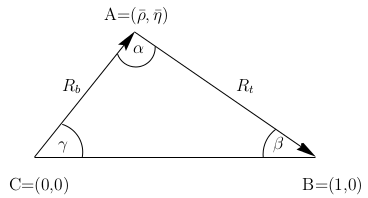
\includegraphics[scale=0.7]{figs/uut.png}
\caption{Unitarity Triangle, using the Wolfenstein parametrization \red{ref, PDG}\label{fig:uut}}
\end{center}
\end{figure}

Experimental measurements help determining the different values for the elements that define the triangle in \ref{fig:uut}. Some of these measurements are $(\Delta M)_d/(\Delta M)_s$ (for $R_t$), $\sin{2\beta}$, $B_d^0\rightarrow \phi K_S^0$ (for $\beta$) and tree-level decays (for $\gamma$).% $K \rightarrow \bar{\pi}\nu\bar{\nu}$, $B \rightarrow X_{d,s} \nu \bar{\nu}$ and $B_{d,s} \rightarrow \mu^+ \mu^-$.  %$\gamma$, tree-level decays 
As said before, NP contributions can affect these values, hence hinting the existence of BSM Physics. 

In order for this triangle to be \textit{universal} to any SM extension, the requirement that new operators don't exist has to be fulfilled. Also, FCNC transitions should be ruled by the CKM eements. \red{Hence, only the values of the functions describing top-medited contributions to box and penguin diagrams can be modified by this new physics ~\cite{Buras:2000dm}.}
Under these conditions, the CKM matrix can be determined without further assumption on the unknown BSM parameters, with the possibility of disentangling SM contributions from NP ones, looking for inconsistencies in the universal triangle or disagreements of the data with respect to the predictions made based on the UUT. As an extra feature, these parameters are not affected by hadronic uncertainties ~\cite{Buras:2000dm}. 

The most up-to-date determination of the elements of the UUT can be found in \ref{fig:uutEXP}. 
\begin{figure} [htb!]
\begin{center}
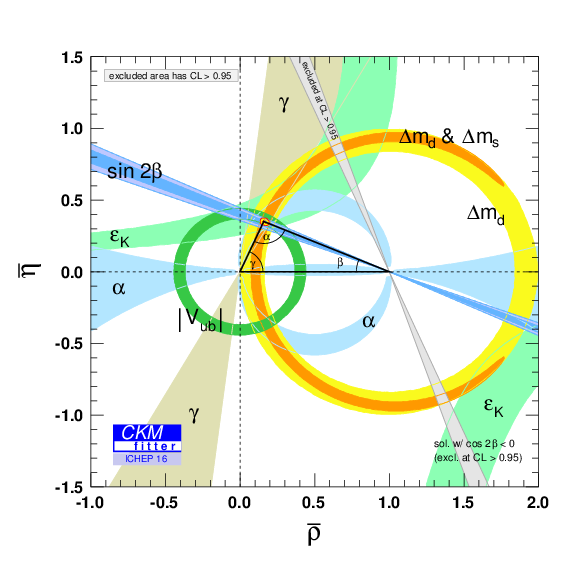
\includegraphics[scale=0.5]{figs/uut_CKMFitter.png}
\caption{Experimental constraints on the UUT, using the Wolfenstein parametrization ~\cite{CKMFitter}\label{fig:uutEXP}}
\end{center}
\end{figure}


\begin{comment}
The SUSY prolem and the MFV principle (Paradisi, Straub): The Bmu term will be complex at the high scale; thi is the approach that is commonly assumed e.g. in the CMSSM
\red{conclusion: not equivalent?}


\end{comment}
~\cite{Fellini4}


